% Leonhard Schatt

\subsection{Lock-in Verstärker}

Der Lock-in Verstärker ist ein wichtiges Messgerät. Er wird dazu verwendet schache Signale, die normalerweise weit unter dem Rauschen liegen noch aufzulösen.
Dabei detektiert das Eingangssignal phasenempfindlich. Beim Messen eines Gleichspannungssignals wir das Signal von einem Chopper in den rauscharmen Bereich "hochgemischt". 
Dies geschieht, da bei niedrigen Frequenzen das "rosa Rauschen" dominiert. (Quelle Herink) 

\begin{figure}[h]
    \centering
    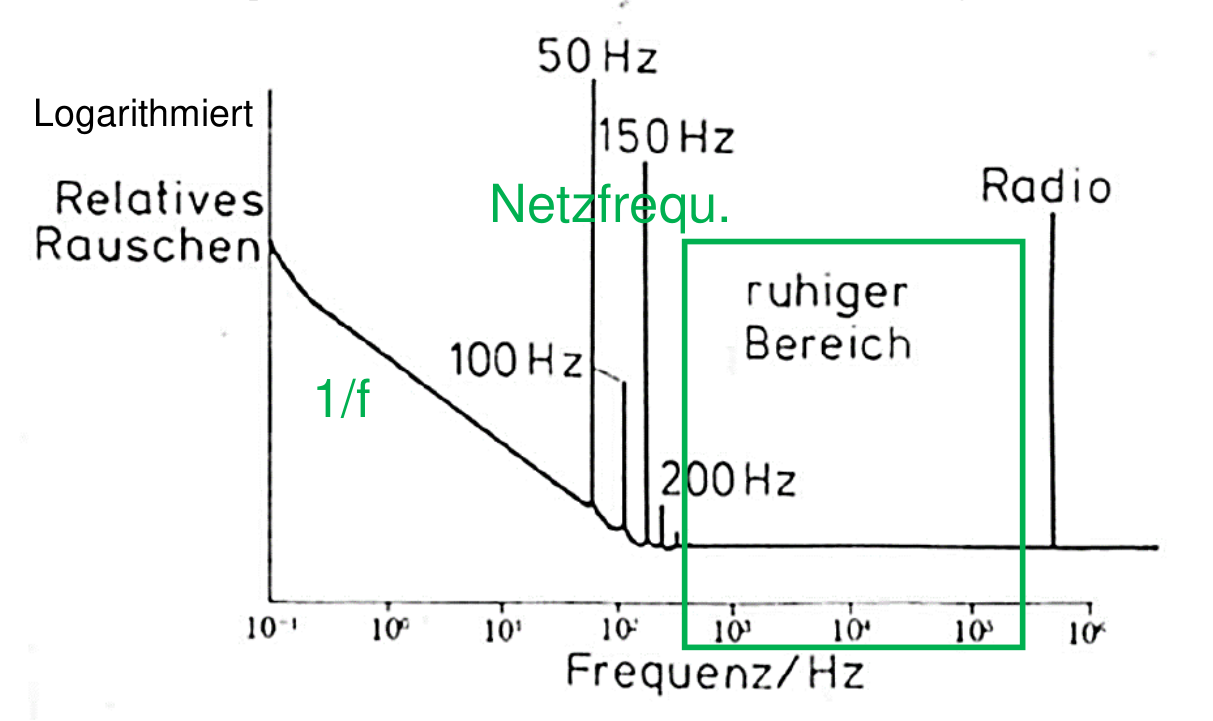
\includegraphics[width = 10cm ]{Bilder/Rauschen.png}
\end{figure}
Im Lock-in Verstärker selbst wird das Signal dann verstärkt und mit einem Referenzsignal $V_R$ gleich der Chopperfrequenz gemischt. Dabei entsteht nach Additiontheoremen für Sinus und Cosinus eine
Differenz- und Summenfrequenz. Dann Filtert man die Differenzfrequenz heraus, indem man einen Tiefpassfilter hinter den Mischer stellt. Im Anschluss wir dann die Spannung abgegriffen. 
Der Vorteil dieses Aufbaus ist, dass die beiden Modulationen durch Chopper und Mischer zusammen wie ein sehr schmalbandiger Filter wirken. Dabei können Bandbreiten von bis zu 0,01Hz erreicht werden. 
Außerdem mittelt sich das Rauschen weg, das es in Beziehung zu $V_R$ unkorreliert ist. Die ausgegebene Spannung hängt jetzt aber noch von der Phasenbeziehung zwischen dem 
modulierten Eingangssignal $V_S$ und dem Referenzsignal $V_R$, das am Mischer ankommt, ab.
\begin{figure}[ht]
    \centering
    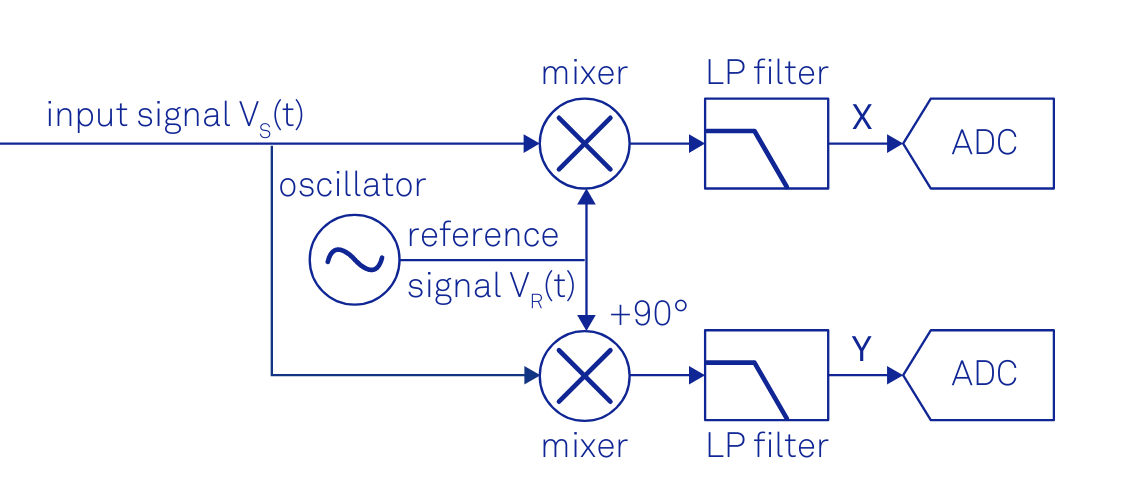
\includegraphics[width = 12cm]{Bilder/Lockin.png}
    \caption{Lock-in Verstärker mit schon moduliertem Eingangssignal $V_S$}
    \label{lockin}
\end{figure}
 Deswegen fügt man, wie in Grafik \ref{lockin} zu sehen, einen zweiten Arm ein, on welchen $V_R$ 
um 90° verzögert wird. Aus den beiden Amplituden $X$ und $Y$ berechnet man dann die Amplitude $R$ des Ausgangssignals folgendermaßen:
\begin{equation*}
    R = \sqrt{X^{2}+Y^{2}}
\end{equation*}
  

